\usetikzlibrary{datavisualization.formats.functions,backgrounds,calc}
\def\mytypesetter#1{% page 813
  \pgfmathparse{#1/pi}%
  \pgfmathprintnumber{\pgfmathresult}$\pi$%
}

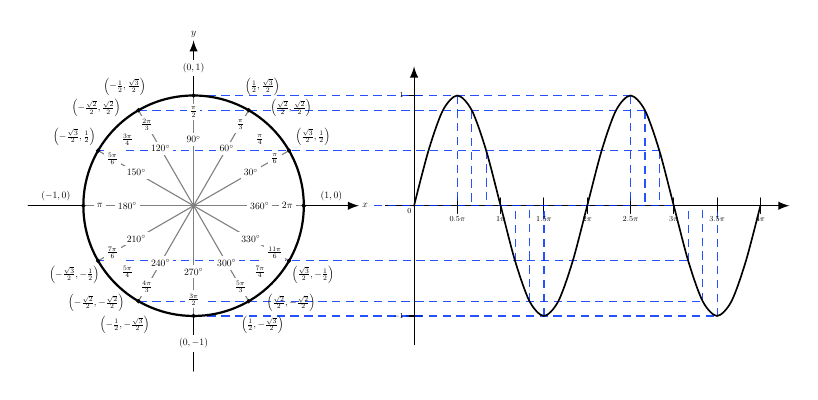
\begin{tikzpicture}[scale=1.4, transform shape, cap=round,>=latex, every node/.style={scale=0.25}] 
\draw[->] (-1.5cm,0cm) -- (1.5cm,0cm) node[right,fill=white] {$x$};
\draw[->] (0cm,-1.5cm) -- (0cm,1.5cm) node[above,fill=white] {$y$};

\draw[thick] (0cm,0cm) circle(1cm);

\foreach \x in {0,30,...,360} {
    \draw[gray] (0cm,0cm) -- (\x:1cm);
    \filldraw[black] (\x:1cm) coordinate (x\x) circle (0.4pt);
    \draw (\x:0.6cm) node[fill=white] {$\x^\circ$};
}

\foreach \x/\xtext in {
    30/\frac{\pi}{6},
    45/\frac{\pi}{4},
    60/\frac{\pi}{3},
    90/\frac{\pi}{2},
    120/\frac{2\pi}{3},
    135/\frac{3\pi}{4},
    150/\frac{5\pi}{6},
    180/\pi,
    210/\frac{7\pi}{6},
    225/\frac{5\pi}{4},
    240/\frac{4\pi}{3},
    270/\frac{3\pi}{2},
    300/\frac{5\pi}{3},
    315/\frac{7\pi}{4},
    330/\frac{11\pi}{6},
    360/2\pi}
\draw (\x:0.85cm) node[fill=white] {$\xtext$};

\foreach \x/\xtext/\y in {
    30/\frac{\sqrt{3}}{2}/\frac{1}{2},
    45/\frac{\sqrt{2}}{2}/\frac{\sqrt{2}}{2},
    60/\frac{1}{2}/\frac{\sqrt{3}}{2},
    150/-\frac{\sqrt{3}}{2}/\frac{1}{2},
    135/-\frac{\sqrt{2}}{2}/\frac{\sqrt{2}}{2},
    120/-\frac{1}{2}/\frac{\sqrt{3}}{2},
    210/-\frac{\sqrt{3}}{2}/-\frac{1}{2},
    225/-\frac{\sqrt{2}}{2}/-\frac{\sqrt{2}}{2},
    240/-\frac{1}{2}/-\frac{\sqrt{3}}{2},
    330/\frac{\sqrt{3}}{2}/-\frac{1}{2},
    315/\frac{\sqrt{2}}{2}/-\frac{\sqrt{2}}{2},
    300/\frac{1}{2}/-\frac{\sqrt{3}}{2}}
\draw (\x:1.25cm) node {$\left(\xtext,\y\right)$};

\draw (-1.25cm,0cm) node[above=1pt] {$(-1,0)$}
(1.25cm,0cm)  node[above=1pt] {$(1,0)$}
(0cm,-1.25cm) node[fill=white] {$(0,-1)$}
(0cm,1.25cm)  node[fill=white] {$(0,1)$};

\begin{scope}[xshift=20mm]
    \datavisualization
    [
    school book axes,
    y axis={unit length=10mm},
    x axis={unit length=2.5mm, ticks={step=(.5*pi), tick typesetter/.code=\mytypesetter{##1}}},
    visualize as smooth line,
    ]
    data [format=function] {
    var x : interval [0:4*pi];
    func y = sin(\value x r);
    };
\end{scope}

\begin{scope}[on background layer]
    \coordinate (o) at (0,0);
    \foreach \i in {90,120,...,270}
    {
        \draw [densely dashed, opacity=.85, color=blue!80!cyan] (x\i) -- ({x\i} -| o) -- ++(20mm,0) -- ++(pi*\i/720,0) coordinate (xx\i) edge (xx\i |- o)  -- ++(.5*pi,0) coordinate (xxx\i) edge (xxx\i |- o);
    }
\end{scope}
\end{tikzpicture}

